%!TEX root = Thesis.tex

\chapter{Sentiment analysis}
\label{chap:sentimentAnalysis}

An continuous analog to the sentiment polarity model presented in the introduction is to weight the classification. Thus the polarity is essential a value in some predefined interval, $[-\omega; \omega]$, as illustrated by Figure~\ref{fig:continuousPolarity}. An opinion with value close to $-\omega$ is considered highly negative, whereas a value close to $\omega$ is considered highly positive. Opinions with values close to zero are considered almost neutral. This model allows the overall process of the sentiment analysis presented by this thesis to be given by Definition~\ref{def:Analysis}.
\begin{figure}[ht]
\begin{center}
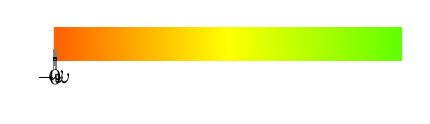
\begin{tikzpicture}
  \pgfdeclarehorizontalshading{myshadingE}{80bp}{color(0bp)=(red!100!white); color(40bp)=(yellow!100!white); color(80bp)=(green!100!white)}   
  \begin{axis}[
    small,
    enlargelimits=0,
    %symbolic x coords={},    
    xtick={-1,0,1},
    xticklabels={$-\omega$,$0$,$\omega$},
    xmin=-1,
    xmax=1,
    %xminorticks=true,
    minor x tick num=3,
    yminorticks=false,
    ymajorticks=false,
    %ytick=\empty,
    %y major tick length=0pt,
    width=6cm,
    height=2cm
  ]
  \addplot[draw=none]{rnd};
  \pgfpathrectangle{\pgfpointorigin}{\pgfpoint{4.425cm}{.42cm}} 
  \pgfshadepath{myshadingE}{0} 
  \end{axis}

\end{tikzpicture}
\end{center}
\vspace{-1em}
\caption{Continuous sentiment polarity model.}
\label{fig:continuousPolarity}
\end{figure}

\begin{definition}
A sentiment analysis $\mathcal{A}$ is a computation on a review text $T \in \Sigma^\star$ with respect to a \emph{subject of interest} $s \in \mathbb{E}$, where $\Sigma^\star$ denotes the set of all texts, and $\mathbb{E}$ is the set of all entities. The result is an normalized score as shown in (\ref{eq:Analysis}). The yielded score should reflect the \emph{polarity} of the given subject of interest in the text, i.e.\ whether the overall opinion is positive, negative, or neutral.
  \begin{align}
	 \mathcal{A}: \Sigma^\star \to \mathbb{E} \to [-\omega;\omega]
	 \label{eq:Analysis}
  \end{align}
  \label{def:Analysis}
  \done
\end{definition}

 It should be evident that this computation is far from trivial, and constitutes the cornerstone of this project. There are several steps needed, if such computation should yield any reasonable result. As mentioned in the introduction the goal is a logical approach for achieving this. The following outlines the overall steps to be completed, their associated problematics in this process, and succinctly presents different approaches to solve each step. The chosen approach for each step will be presented in much more details in later chapters. %Finally TODO: Something about data acquisition of test-data

\section{Tokenization}
\label{sec:tokenization}
In order to even start processing natural language texts, it is essential to be able to identify the elementary parts, i.e.\ \emph{lexical units} and \emph{punctuation marks}, that constitutes a text. Decent tokenization is essential for all subsequent steps. However even identifying the different sentences in a text can yield a difficult task. Consider for instance the text~(\ref{ex:sentenceBoundary}) which is taken from the Wall Street Journal (WSJ) corpus \cite{wsjCorpus}. There are six periods in it, but only two of them indicates sentence boundaries, and delimits the text into its two sentences.

\begin{numquote}
  Pierre Vinken, 61 years old, will join the board as a nonexecutive director Nov. 29. Mr. Vinken is chairman of Elsevier N.V., the Dutch publishing group.  
  \label{ex:sentenceBoundary}
\end{numquote}

The domain of small review texts allows some restrictions and assumptions, that at least will ease this issue. For instance it is argued that the review texts will be fairly succinct, and thus it seems like a valid assumption that they will consists of only a few sentences. Its is argued that this indeed is achievable by sufficient instructing and constraining the reviewers doing data collection, e.g.\ only allowing up to a certain number of characters. This allows sentences in such phrases to be processed independently (i.e.\ as two separate review texts).

Even with this assumption, the process of identifying the sentences, and the lexical units and punctuation marks within them, is not a trivial task. \citeauthor{tokenization}\shortcite{tokenization} criticizes the neglection of this process, as most natural language processing (NLP) studies focus purely on analysis, and assumes this process has already been performed. Such common assumptions might derive from English being a relatively easy language to tokenize. This is due to its space marks as explicit delimiters between words, as opposed to other languages, e.g.\ Chinese which has no delimiters at all. This might hint that tokenization is very language dependent. And even though English is considered simple to tokenize, a naive approach like segmenting by the occurrence of spaces fails for the text~(\ref{ex:lexicalUnitIdentification}), which is also from the WSJ corpus, as it would yield lexical units such as ``(or'', ``perceived,'' and ``rate),''. Simply consider all groups of non-alphanumerics as punctuation marks does not work either, since this would fail for i.a.\ ordinal numbers, currency symbols, and abbreviations, e.g.\ ``Nov.'' and ``Elsevier N.V.'' in text~(\ref{ex:sentenceBoundary}). Both of these methods also fail to recognize ``Pierre Vinken'' and ``Elsevier N.V.'' as single proper noun units, which is arguably the most sane choice for such. 

\begin{numquote1}
One of the fastest growing segments of the wine market is the category of superpremiums -- wines limited in production, of exceptional quality (or so perceived, at any rate), and with exceedingly high prices.
  \label{ex:lexicalUnitIdentification}
\end{numquote1}

\citeauthor{freeLing} \shortcite{freeLing} presents a framework of analytic tools, developed in the recent years, for various NLP tasks. Specially interesting is the morphological analyzer, which applies a cascade of specialized (i.e.\ language dependent) processors to solve exactly the tokenization. The most simple of them use pattern matching algorithms to recognize numbers, dates, quantity expressions (e.g.\ ratios, percentages and monetary amounts), etc. More advanced processing are needed for proper nouns, which relies on a two-level solution: first it applies a fast pattern matching, utilizing that proper nouns are mostly capitalized; and secondly statistical classifiers are applied as described by \citeauthor{adaBoost}~\shortcite{adaBoost}. These recognize proper nouns with accuracy of respectively 90\% and over 92\%. The analyzer also tries to identify lexical units that are composed of multiple words, e.g. proper nouns and idioms.

It is thus possible, by the use of this framework, to preprocess the raw review texts collected from users, and ensure that they will be tokenized into segments that are suitable for the lexical-syntactic analysis. Thus more details on the tokenizer will not be presented.
\vspace{-.5em}

\section{Lexical-syntactic analysis}
\label{sec:syntacticAnalysis}
The syntactic analysis determines the grammatical structure of the input texts with respect to the rules of the English language. It is expected that the reader is familiar with English grammar rules and syntactic categories, including phrasal categories and lexical categories (also called parts of speech). As mentioned earlier it is essential that the presented method is able to cope with \emph{real} data, collected from actual review scenarios. This implies a robust syntactic analysis, accepting a large vocabulary and a wide range of sentence structures. In order to calculate the actual polarity it is essential to have semantic annotations on the lexical units. It is argued that a feasible and suitable solution is to use a grammar that is \emph{lexicalized}, i.e.\ where the rules are essentially language independent, and the syntactic properties are derived from a lexicon. Thus the development of a lexicalized grammar is mainly a task of acquiring a suitable lexicon for the desired language.

Even though the task of syntactic analysis now is largely reduced to a task of lexicon acquisition, which will be addressed in Chapter~\ref{chap:lexiconAcquisition}, there are still general concerns that are worth acknowledging. \citeauthor{extendingCCG}~\shortcite[p.~108-110]{extendingCCG}\ identifies several issues in being able to efficiently handle natural language texts solely with lexicalized grammars, mainly due to the need for entries for various combinations of proper nouns, abbreviated terms, dates, numbers, etc. Instead they suggest to use pattern matching and statistical techniques as a preprocessing step, for which efficient components exists, which translate into reduced complexity for the actual syntactic analysis. The tokenization framework \cite{freeLing} introduced in the previous section does exactly such kind of identification, and thus this should not yield significant problems. 

However the domain of small review texts also introduce problematics that may not an constitute major concerns in other domains, most notable the possibility of incorrect grammar and spelling, since the texts comes unedited from humans with varying English skills. Recall from the Section \label{sec:realData} that a solution that only would work on \emph{perfect texts} (i.e.\ texts of sentences with completely correct grammar and spelling) would not be adequate. The grammar shoulf at least be able to handle minor misspellings. Reasons for this could be that word is simply absent  from the system's vocabulary (e.g.\ misspelled), or on a grammatical incorrect form (e.g.\ wrong person, gender, tense, case, etc.). 

\section{Mildly context-sensitive grammars}
There exists formal proofs that some natural language structures requires formal power beyond \emph{context-free grammars} (CFG), i.e.\ \cite{nlpNotCFG} and \cite{nlpNotCFG2}. Thus the search for grammars with more expressive power has long been a major study within the field of computational linguistics. The goal is a grammar that is so restrictive as possible, allowing efficient syntactic analysis, but still capable of capturing these structures. The class of \emph{mildly context-sensitive grammars} are conjectured to be powerful enough to model natural languages while remaining efficient with respect to syntactic analysis cf. \cite{mildlyCSG}.

Different grammar formalisms from this class has been considered, including \emph{Tree Adjunct Grammar} (TAG) \cite{tag}, in its lexicalized form (LTAG), \emph{Head Grammar} (HG) \cite{hg} and \emph{Combinatory Categorial Grammar} (CCG) \cite{steedmanDraft}. It has been shown that these are all equal in expressive power by \citeauthor{theEquivalence}~\shortcite{theEquivalence}. The grammar formalism chosen for the purpose of this thesis is \emph{Combinatory Categorial Grammar} (CCG), pioneered largely by \citeauthor{sp}~\shortcite{sp}. CCG adds a layer of combinatory logic onto pure Categorial Grammar, which allows an elegant and succinct formation of \emph{higher-order} semantic expressions directly from the syntactic analysis. Since the goal of this thesis is a logical approach to sentiment analysis, CCG's native use of combinatory logic seemed like the most reasonable choice. Chapter~\ref{chap:ccg} will formally introduce the CCG in much more detail.

\section{Semantic analysis}
\label{sec:semanticAnalysis}
The overall process of semantic analysis in the context of sentiment analysis is to identify the polarity of the entities appearing in the text, and to relate these entities to the \emph{subject of interest} of the sentiment analysis. The approach is to \emph{annotate} the lexical units of adjectives and adverbs with suitable polarities, and then fold these onto the phrasal structures, yielded by the syntactic analysis, in order to identify the bindings of these polarities, i.e.\ which entities they modify directly or indirectly.

There exists datasets that tries to bind a general polarity to each word in a lexicon, e.g.\ \cite{sentiWordNet} and \cite{sentiWordNet3}. While such might be fine for general sentiment analyses, or analyses where the domain is not known, it is argued that better results can be achieved by using a domain specific annotation. For instance the adjective ``huge'' might be considered positive for a review describing rooms at a hotel, while negative for a review describing sizes of cell phones.

As already mentioned, the use of a lexicalized syntactic analysis allows the annotation to appear directly on the entries in the lexicon. A manual annotation of a large lexicon is evidently not a feasible approach. Furthermore the model must also be generic enough so it can be adapted to ideally any domain contexts with minimum efforts, i.e.\ it is not desired to tie the model to any specific domain, or type of domains. To achieve such a model that is loosely coupled to the domain the concept of \emph{semantics networks} was chosen cf.\ \citeauthor{ai} \shortcite[p.~454--456]{ai}.

A semantic network is in its simplest form just a collection of different semantic concepts, and relations between them. The idea is to dynamically construct such semantic networks from a small set of domain specific knowledge, namely a set of positive and negative \emph{seed concepts} in the domain -- a technique presented by \citeauthor{valenceShifting} \shortcite{valenceShifting}. Section~\ref{sec:sentimentValue} in Chapter~\ref{chap:lexiconAcquisition} will presents details on the approach of calculating the polarities of adjectives and adverbs and additionally present some handling of negations.

The final result of the sentiment analysis is simply the aggregation of the results yielded for each of the results of the semantic analysis.